\documentclass[tikz,border=3.14mm]{standalone}
\usetikzlibrary{positioning}

\begin{document}
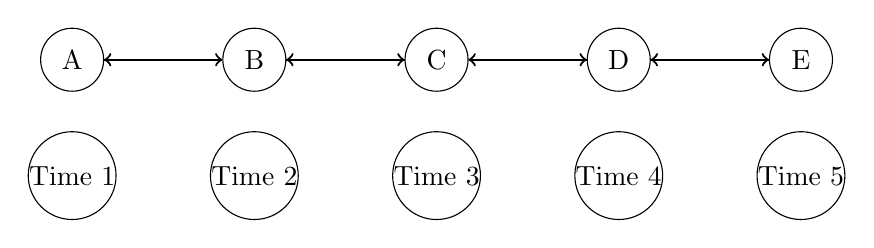
\begin{tikzpicture}[
    node distance=1.5cm,
    every node/.style={circle, draw, minimum size=0.8cm, inner sep=0}
]
    % Nodes
    \node (A) {A};
    \node (B) [right=of A] {B};
    \node (C) [right=of B] {C};
    \node (D) [right=of C] {D};
    \node (E) [right=of D] {E};
    
    % Bold edges (expected, consecutive forward)
    \draw[thick, ->] (A) -- (B);
    \draw[thick, ->] (B) -- (C);
    \draw[thick, ->] (C) -- (D);
    \draw[thick, ->] (D) -- (E);
    
    % Dotted edges (implausible, backward)
    \draw[dotted, thick, ->] (B) -- (A);
    \draw[dotted, thick, ->] (C) -- (B);
    \draw[dotted, thick, ->] (D) -- (C);
    \draw[dotted, thick, ->] (E) -- (D);
    
    % Optional: Add labels for clarity
    \node[below=0.5cm of A, anchor=north] {Time 1};
    \node[below=0.5cm of B, anchor=north] {Time 2};
    \node[below=0.5cm of C, anchor=north] {Time 3};
    \node[below=0.5cm of D, anchor=north] {Time 4};
    \node[below=0.5cm of E, anchor=north] {Time 5};
\end{tikzpicture}
\end{document}